\documentclass[12pt]{article}

\usepackage{graphicx}

\begin{document}

%Below we make use of the graphicx package.
%Note that it doesn't work on the standard .dvi build. You need to compile
%using pdflatex.
%Image names should not include spaces. If they do, you will need to encapsulate
%them in double quotes.
%This is considered the best way as you're controlling the width of the image in
%proportion to the textwidth. Too much guess work in the other methods.
\begin{center}
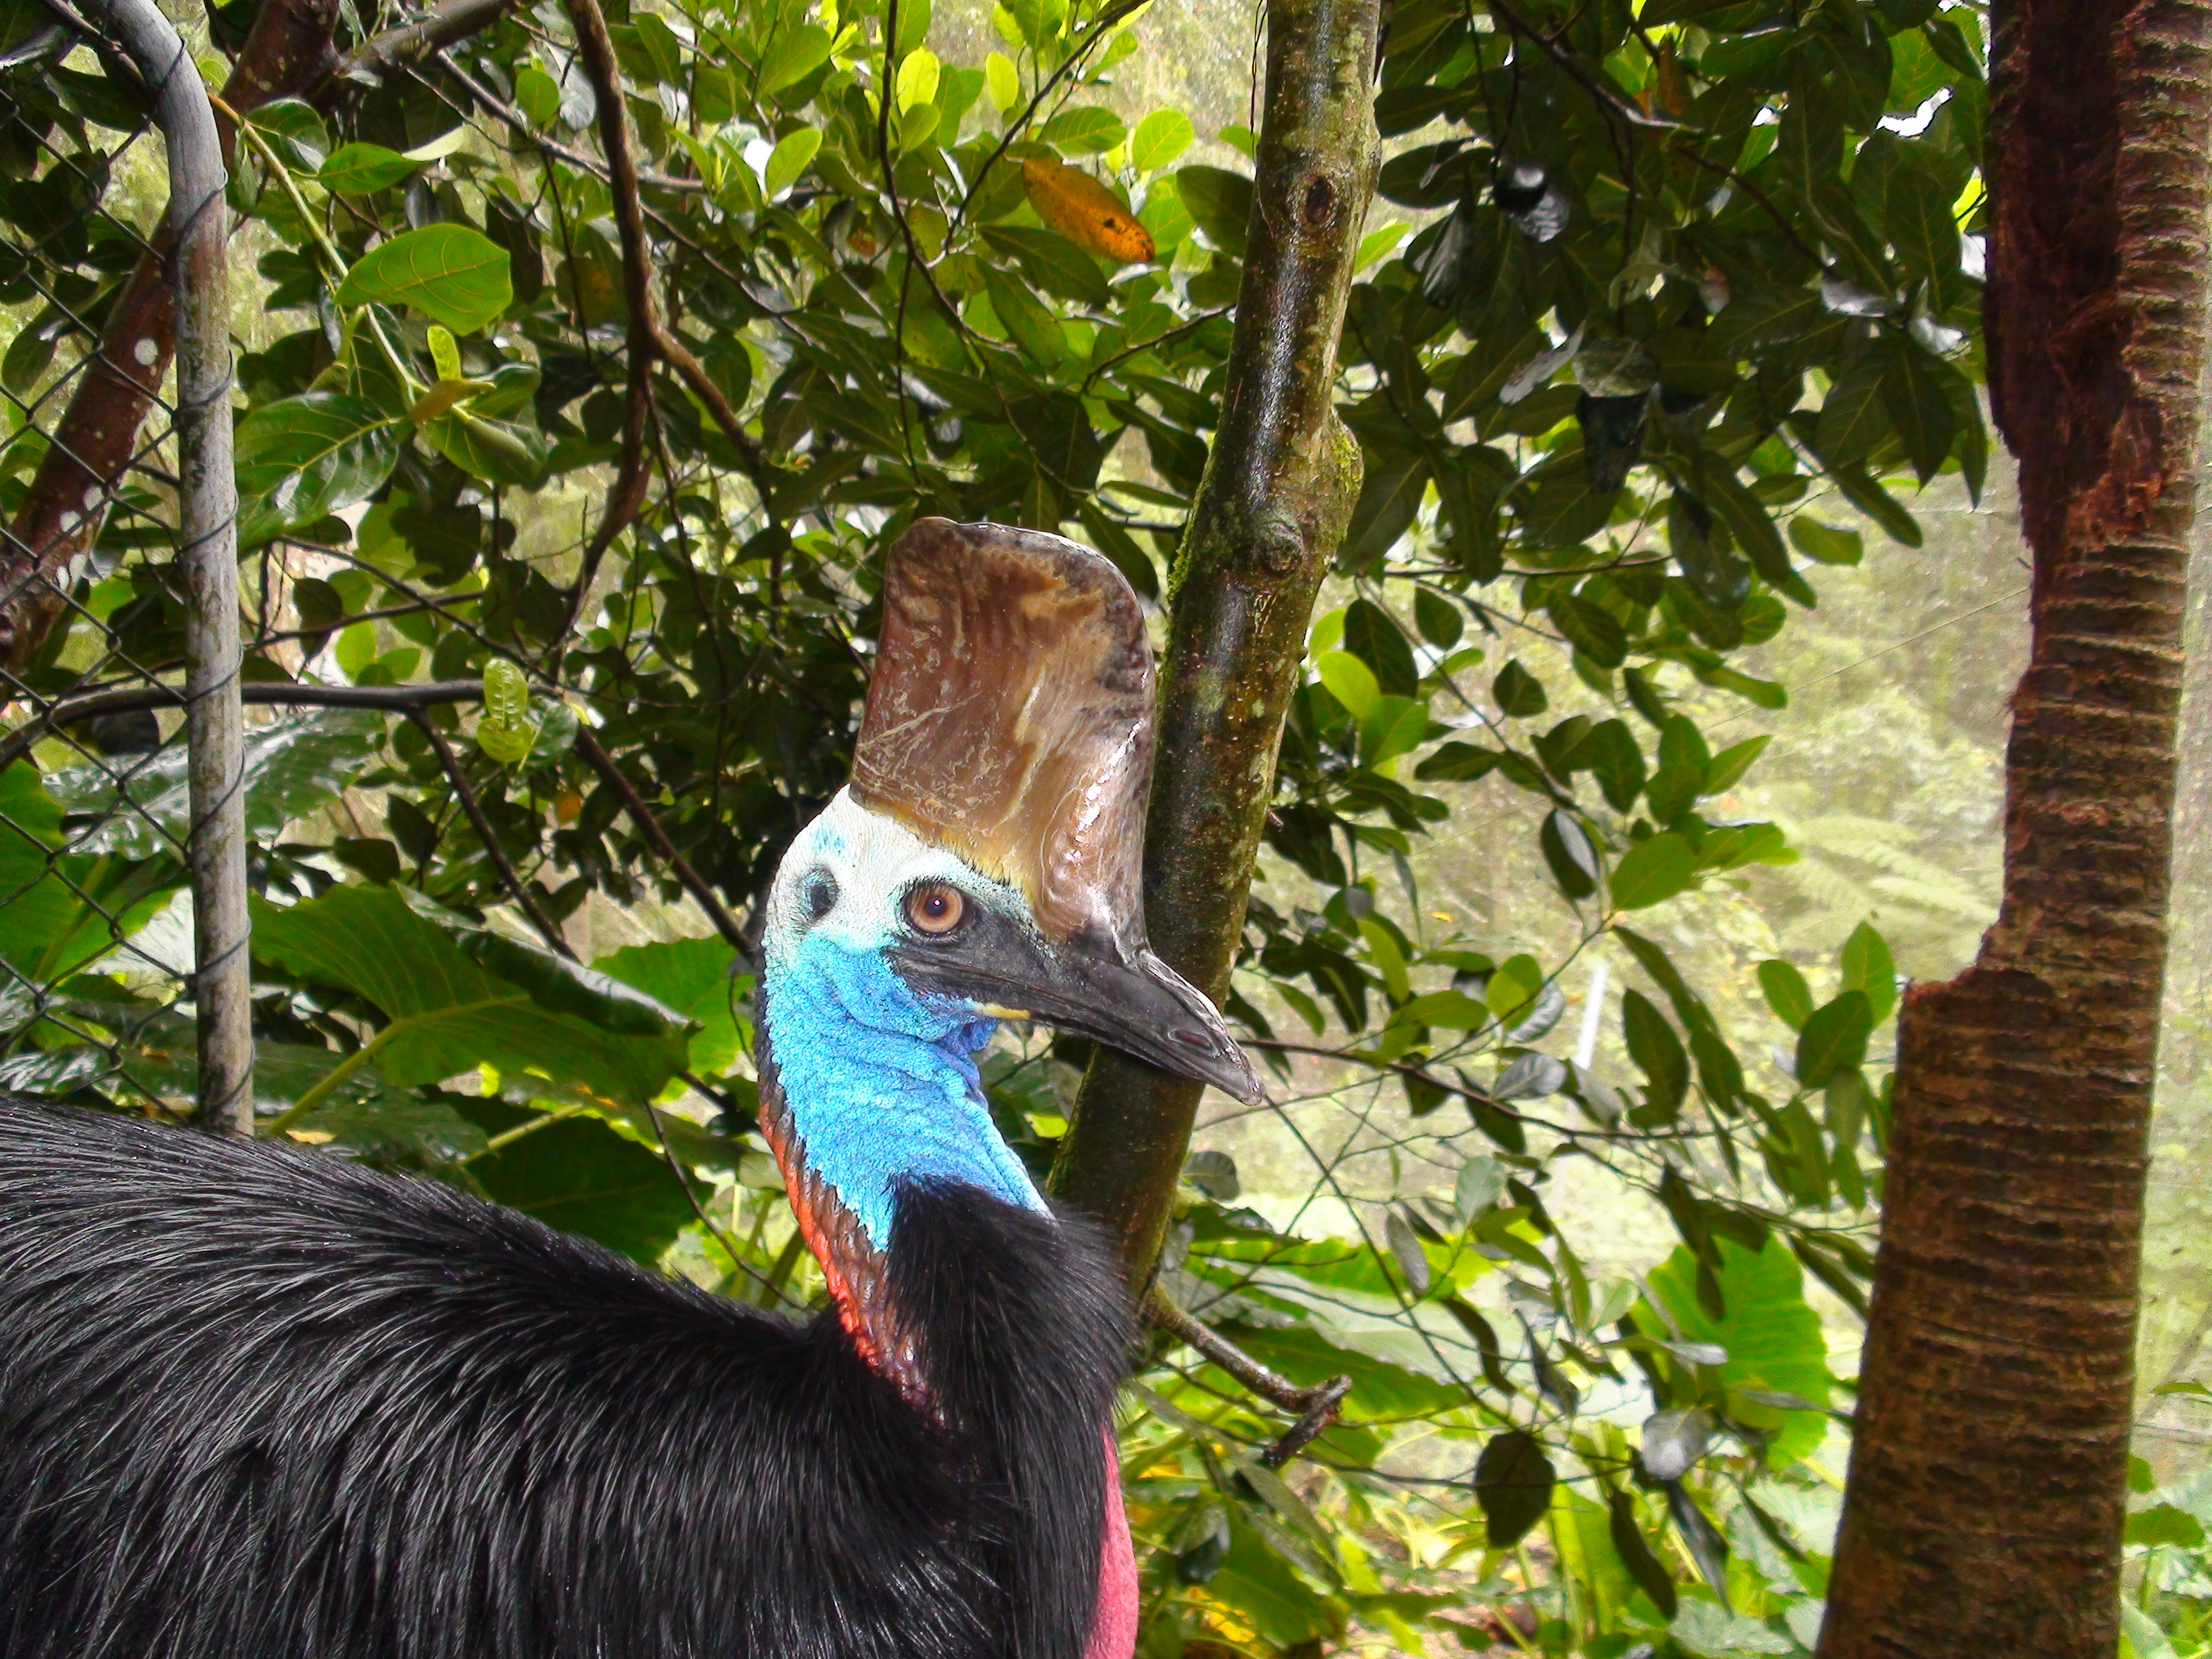
\includegraphics[width=0.8\textwidth]{bird}
\end{center}

\begin{center}
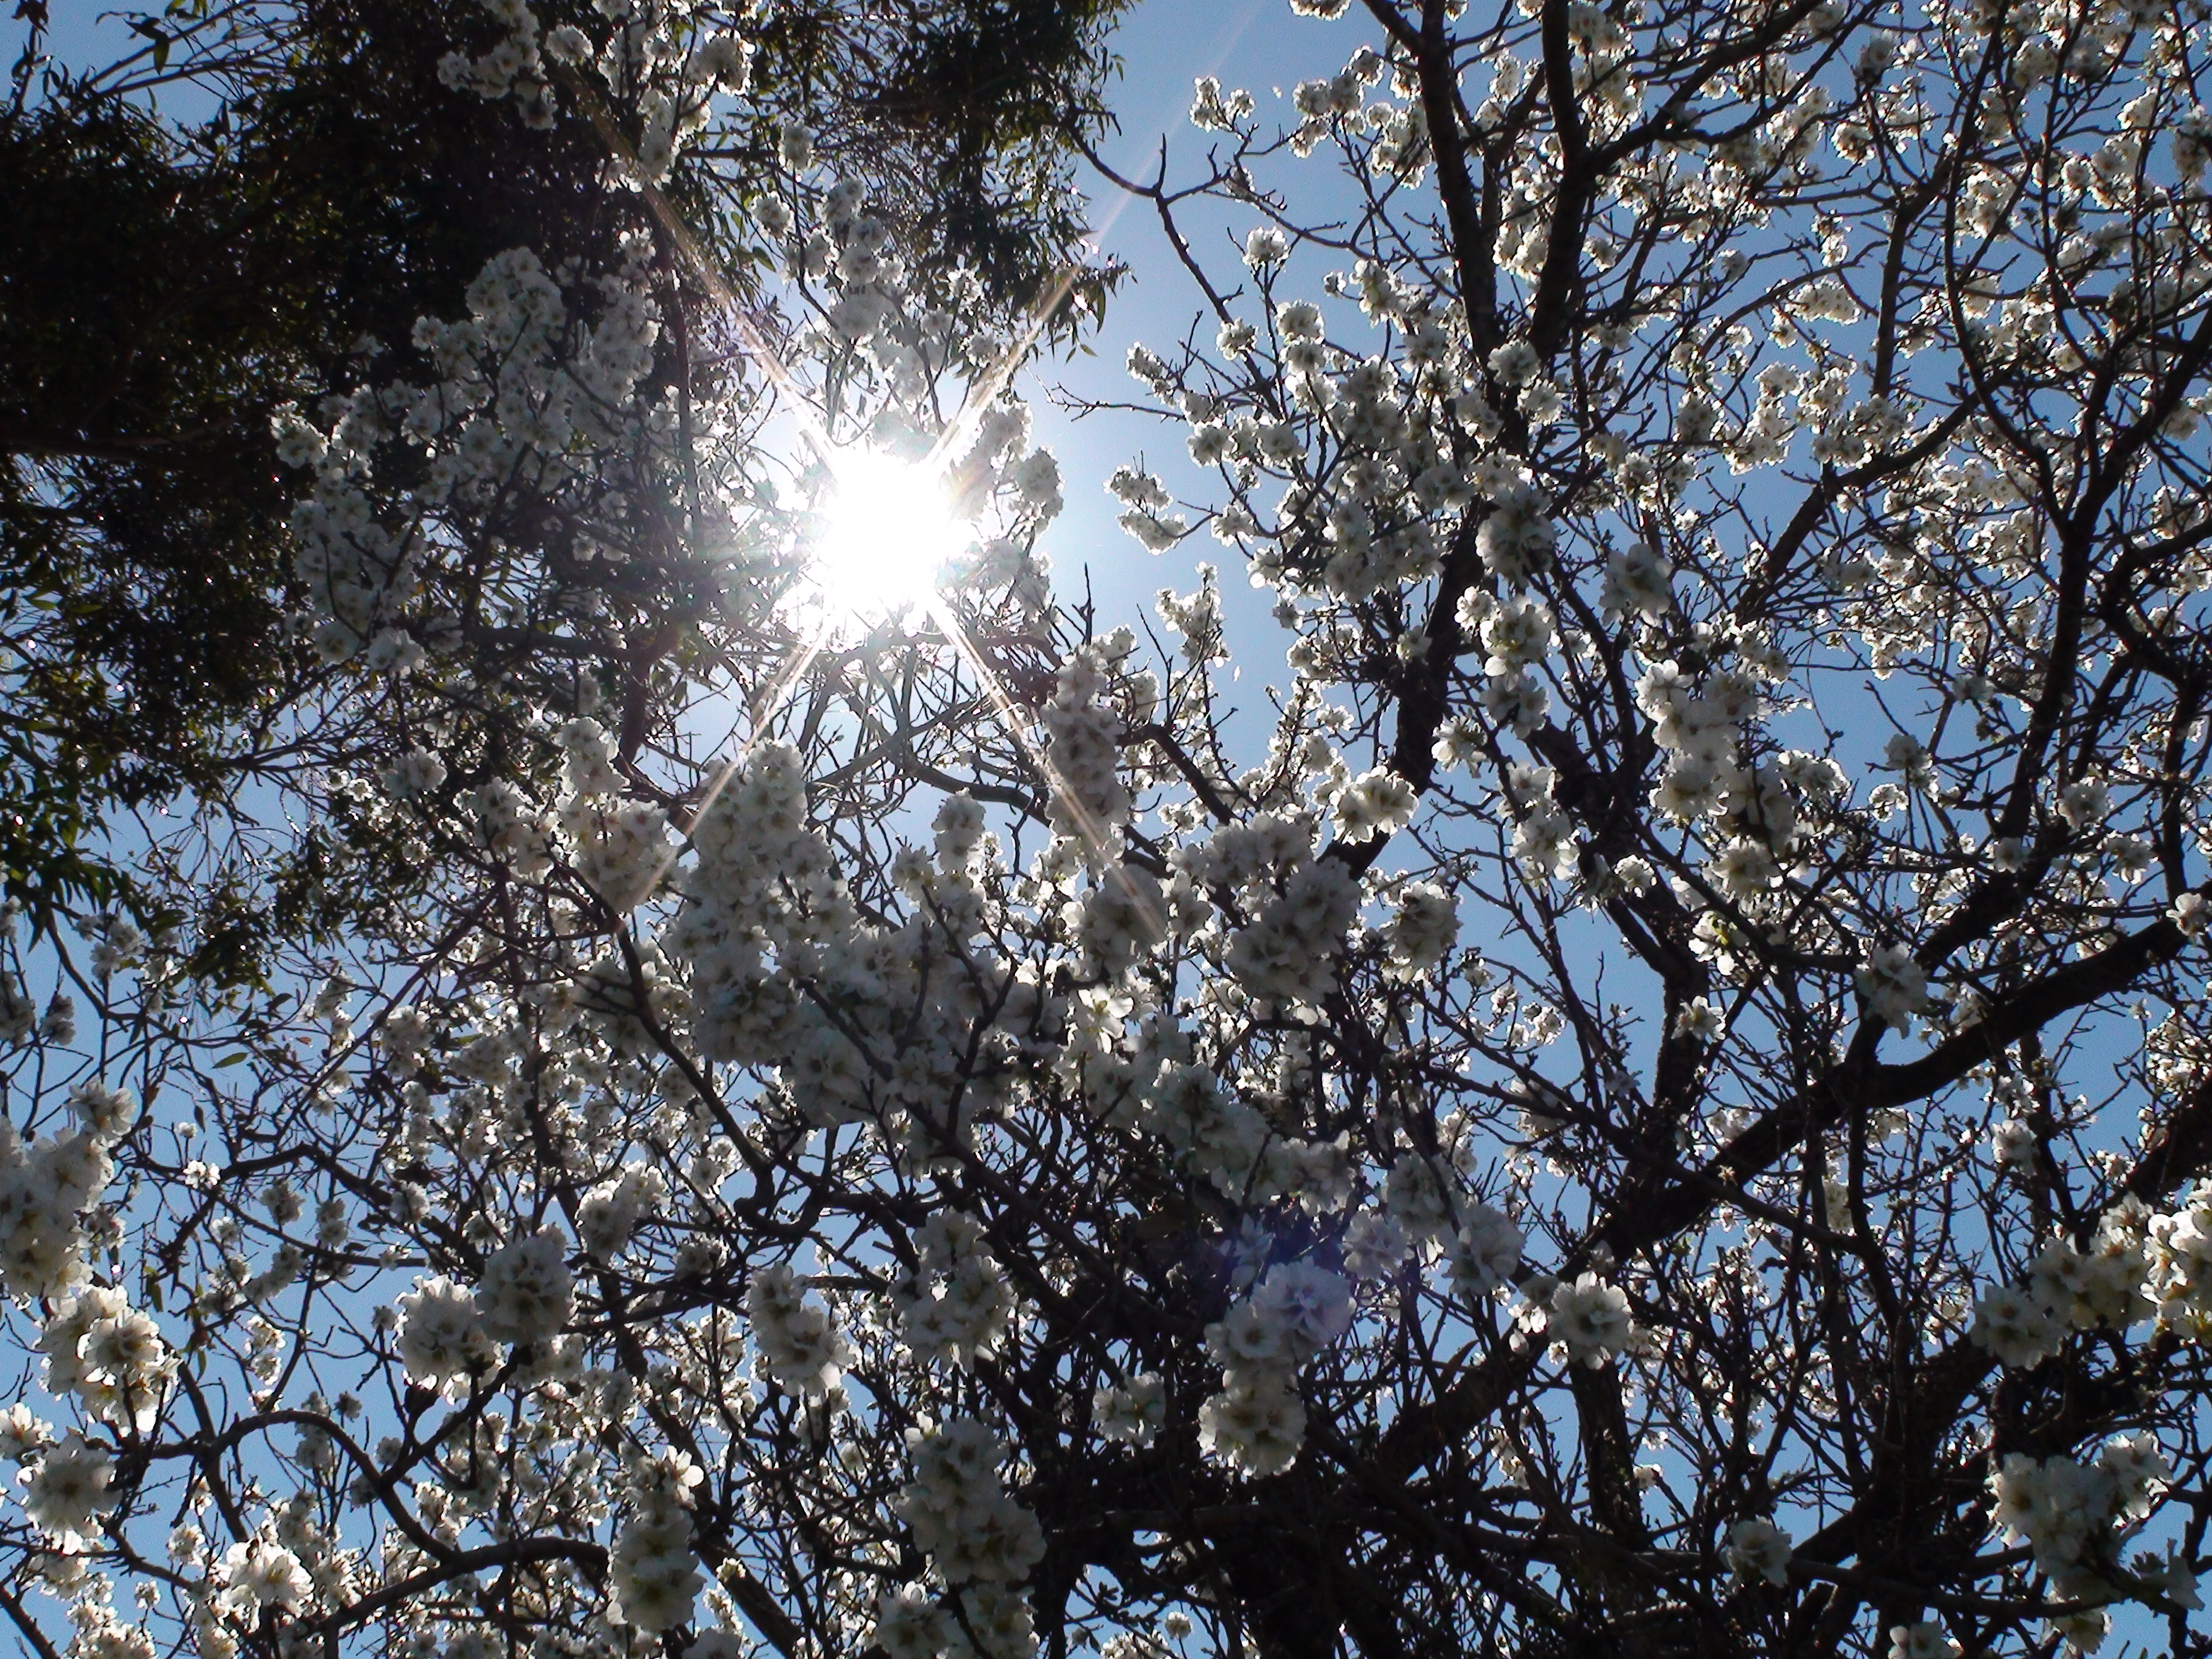
\includegraphics[width=5in]{tree}
\end{center}

\begin{flushright}
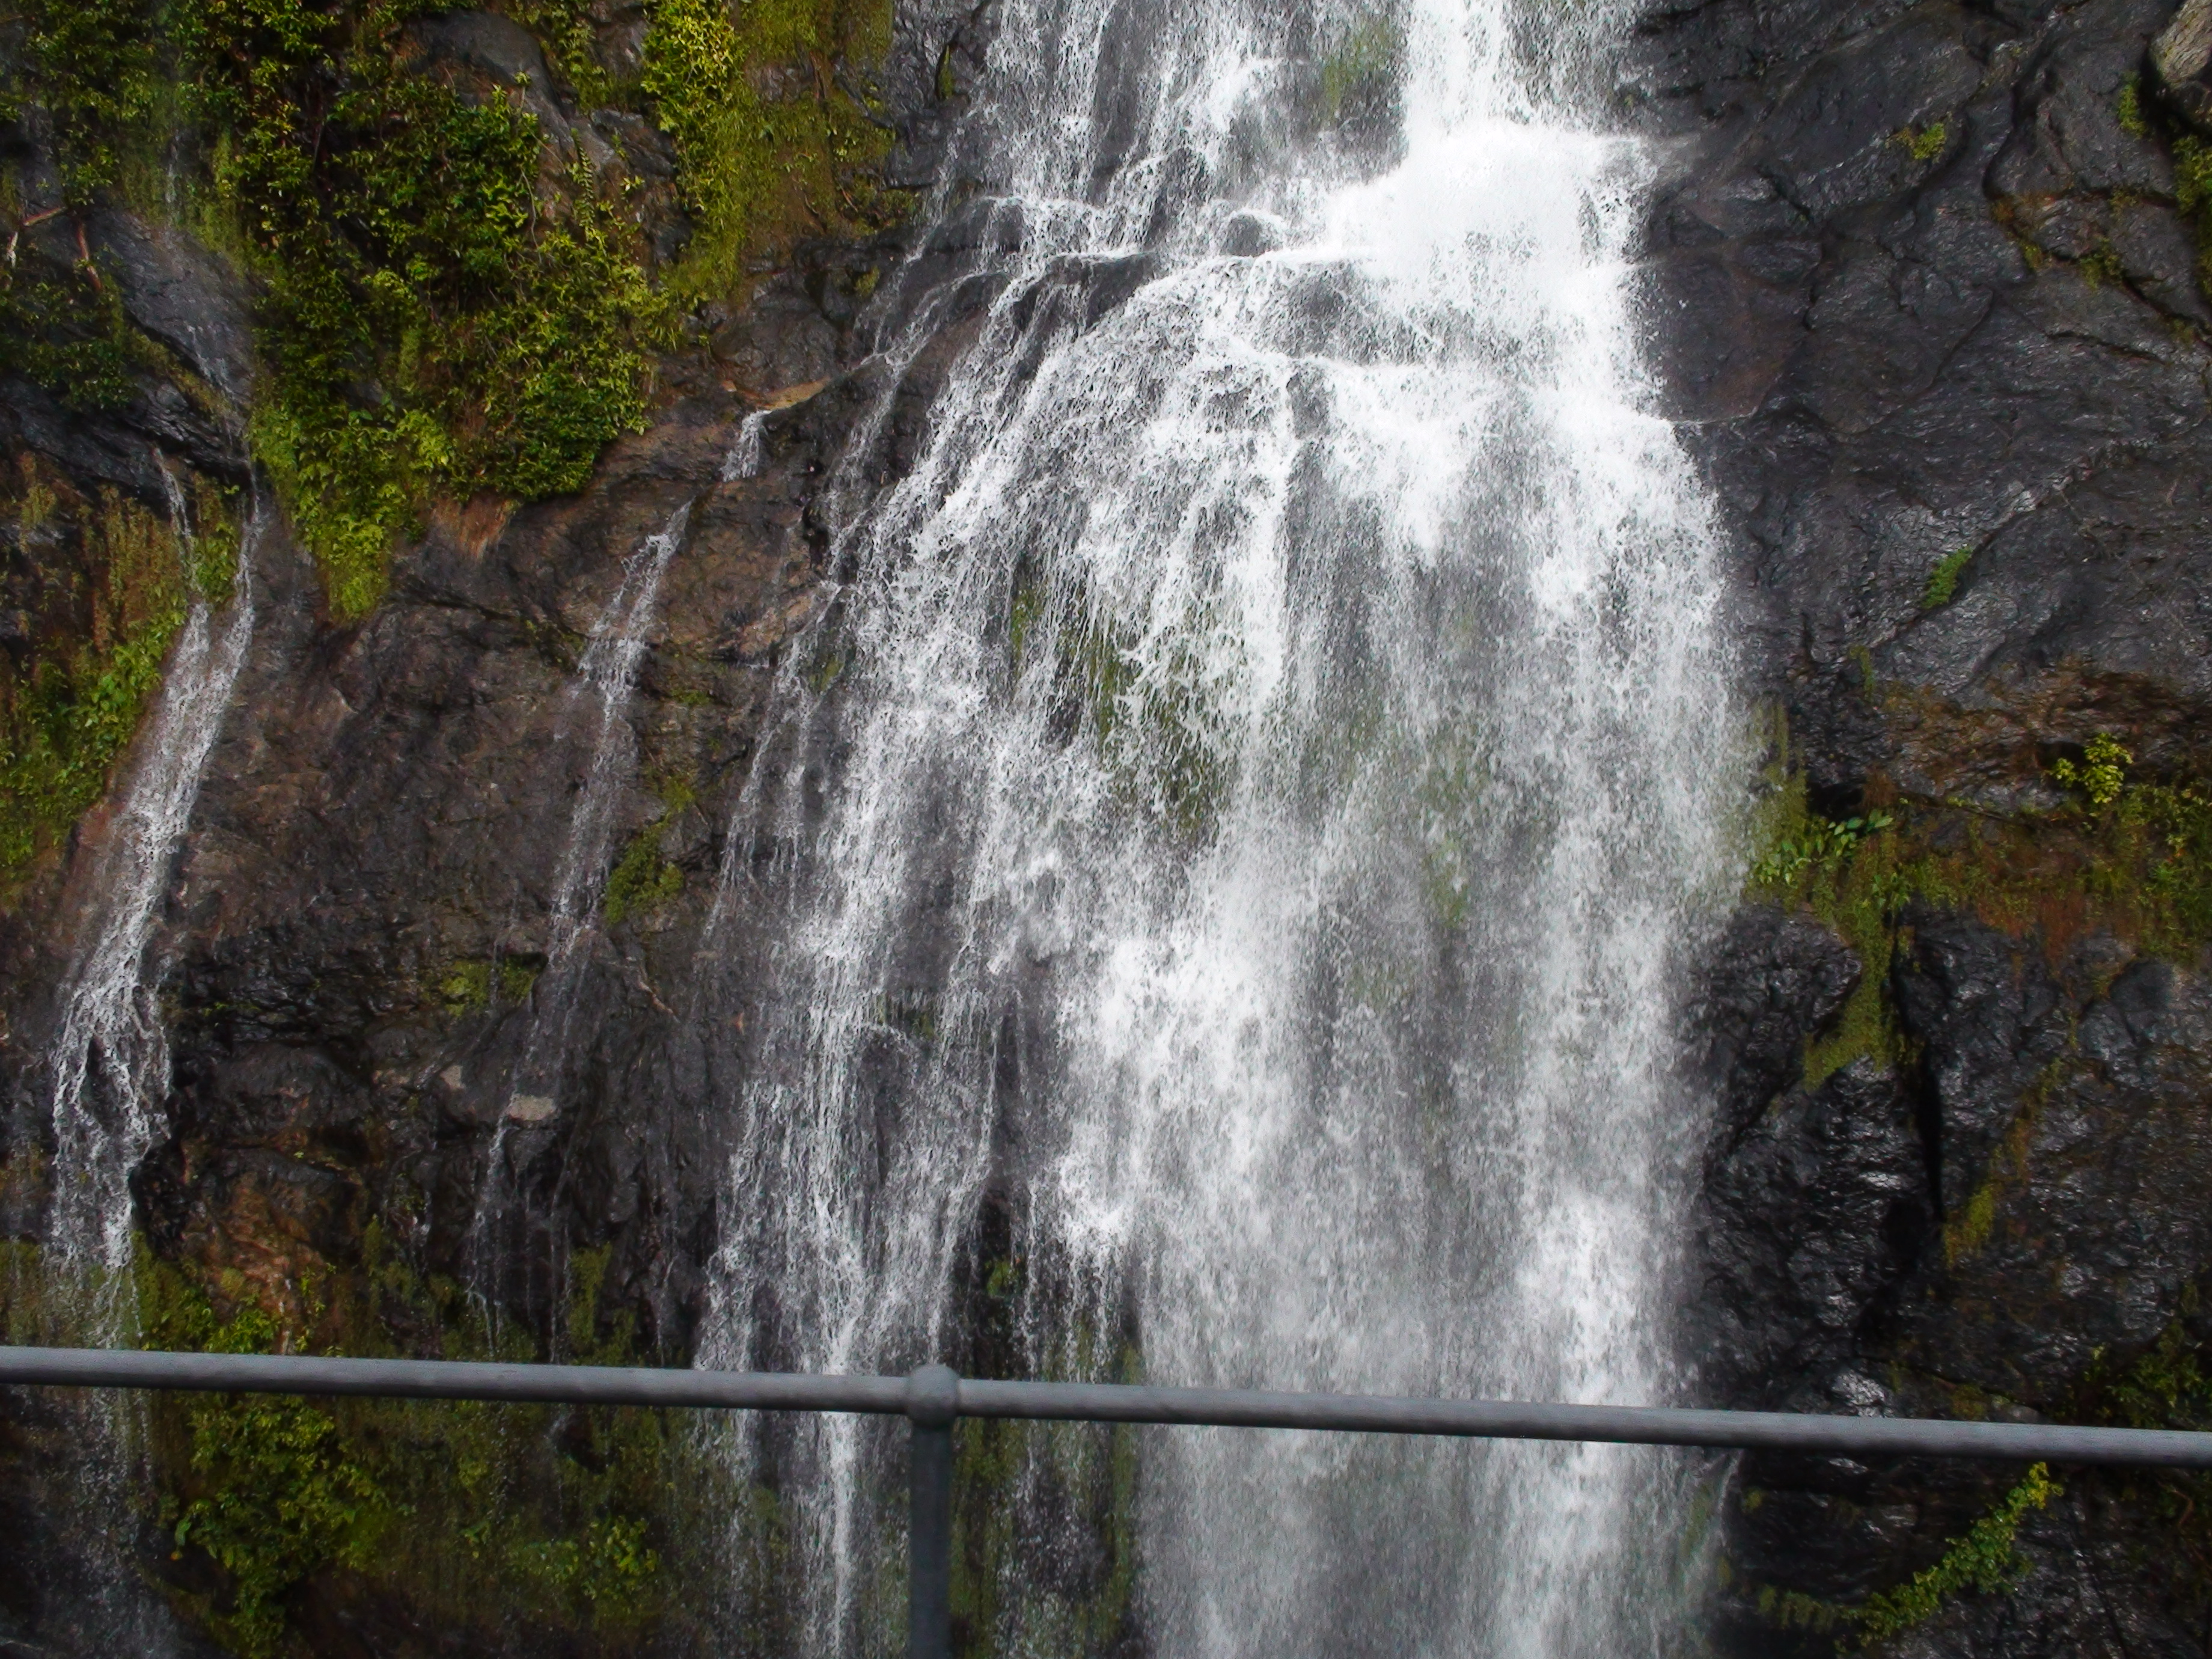
\includegraphics[scale=0.07]{waterfall}
\end{flushright}

\begin{flushleft}
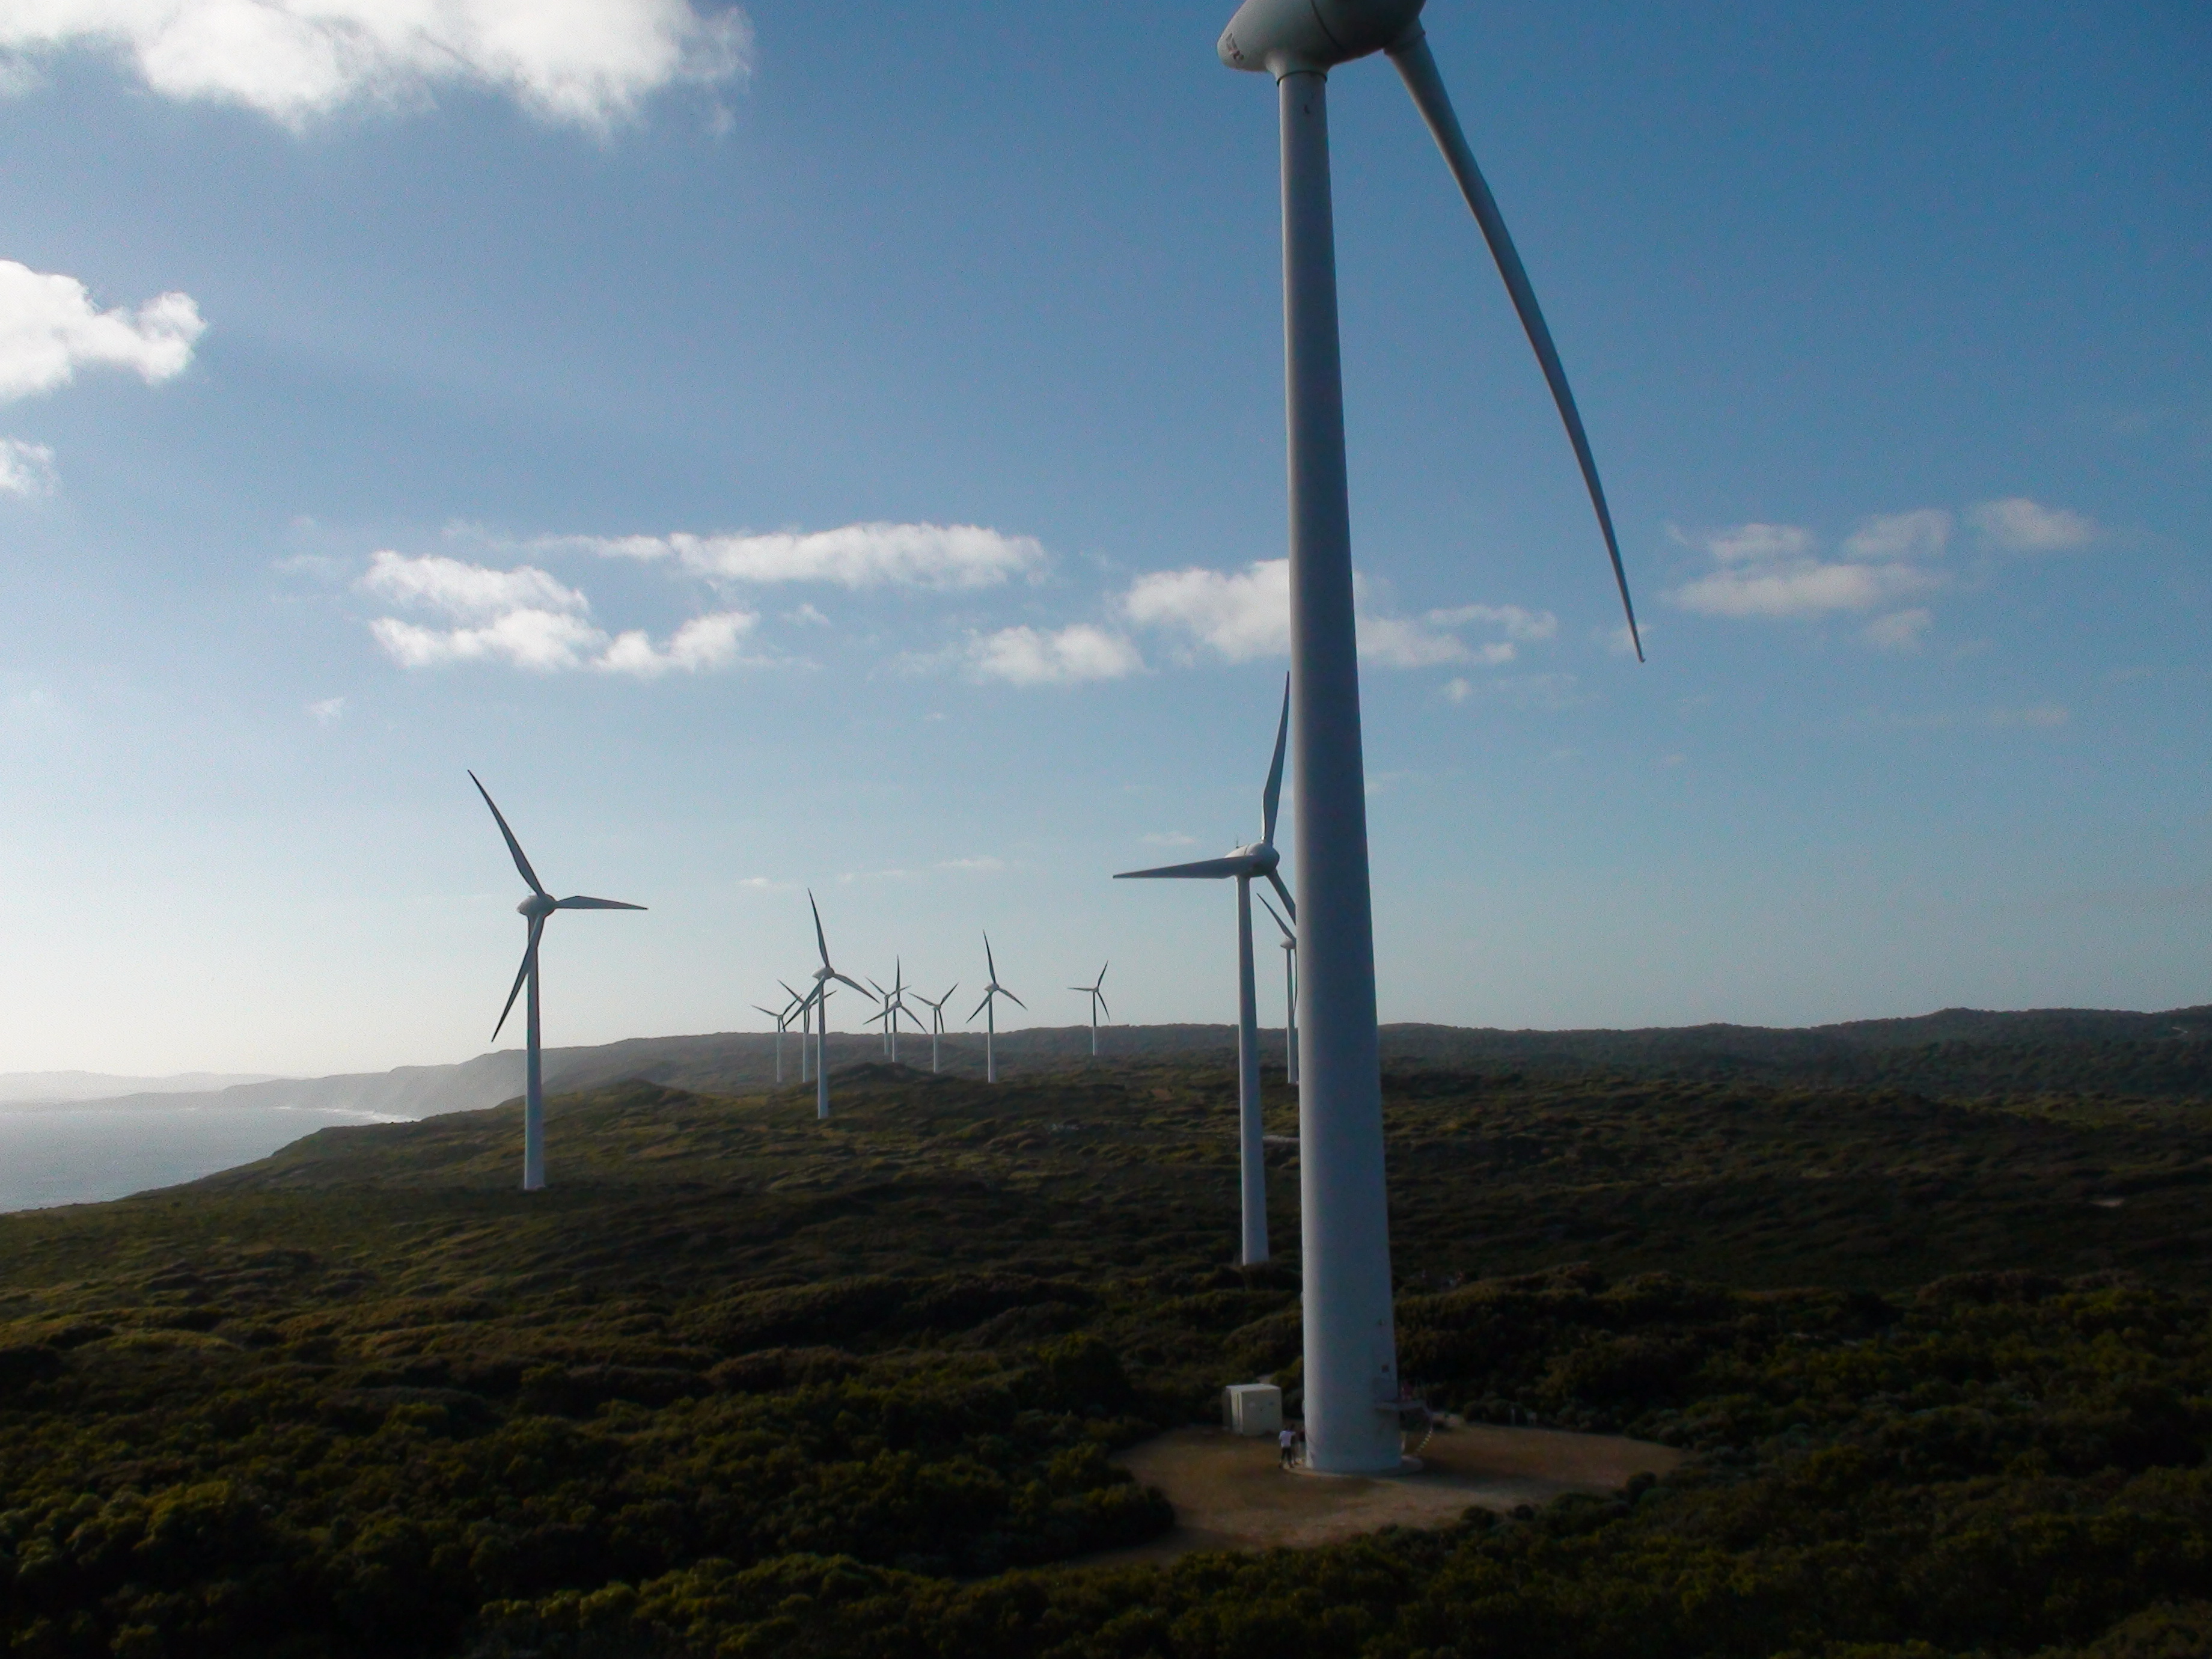
\includegraphics[scale=0.07]{windmill}
\end{flushleft}

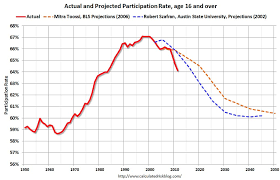
\includegraphics[width=3in]{graph}

%This rotates the image 45 degrees.
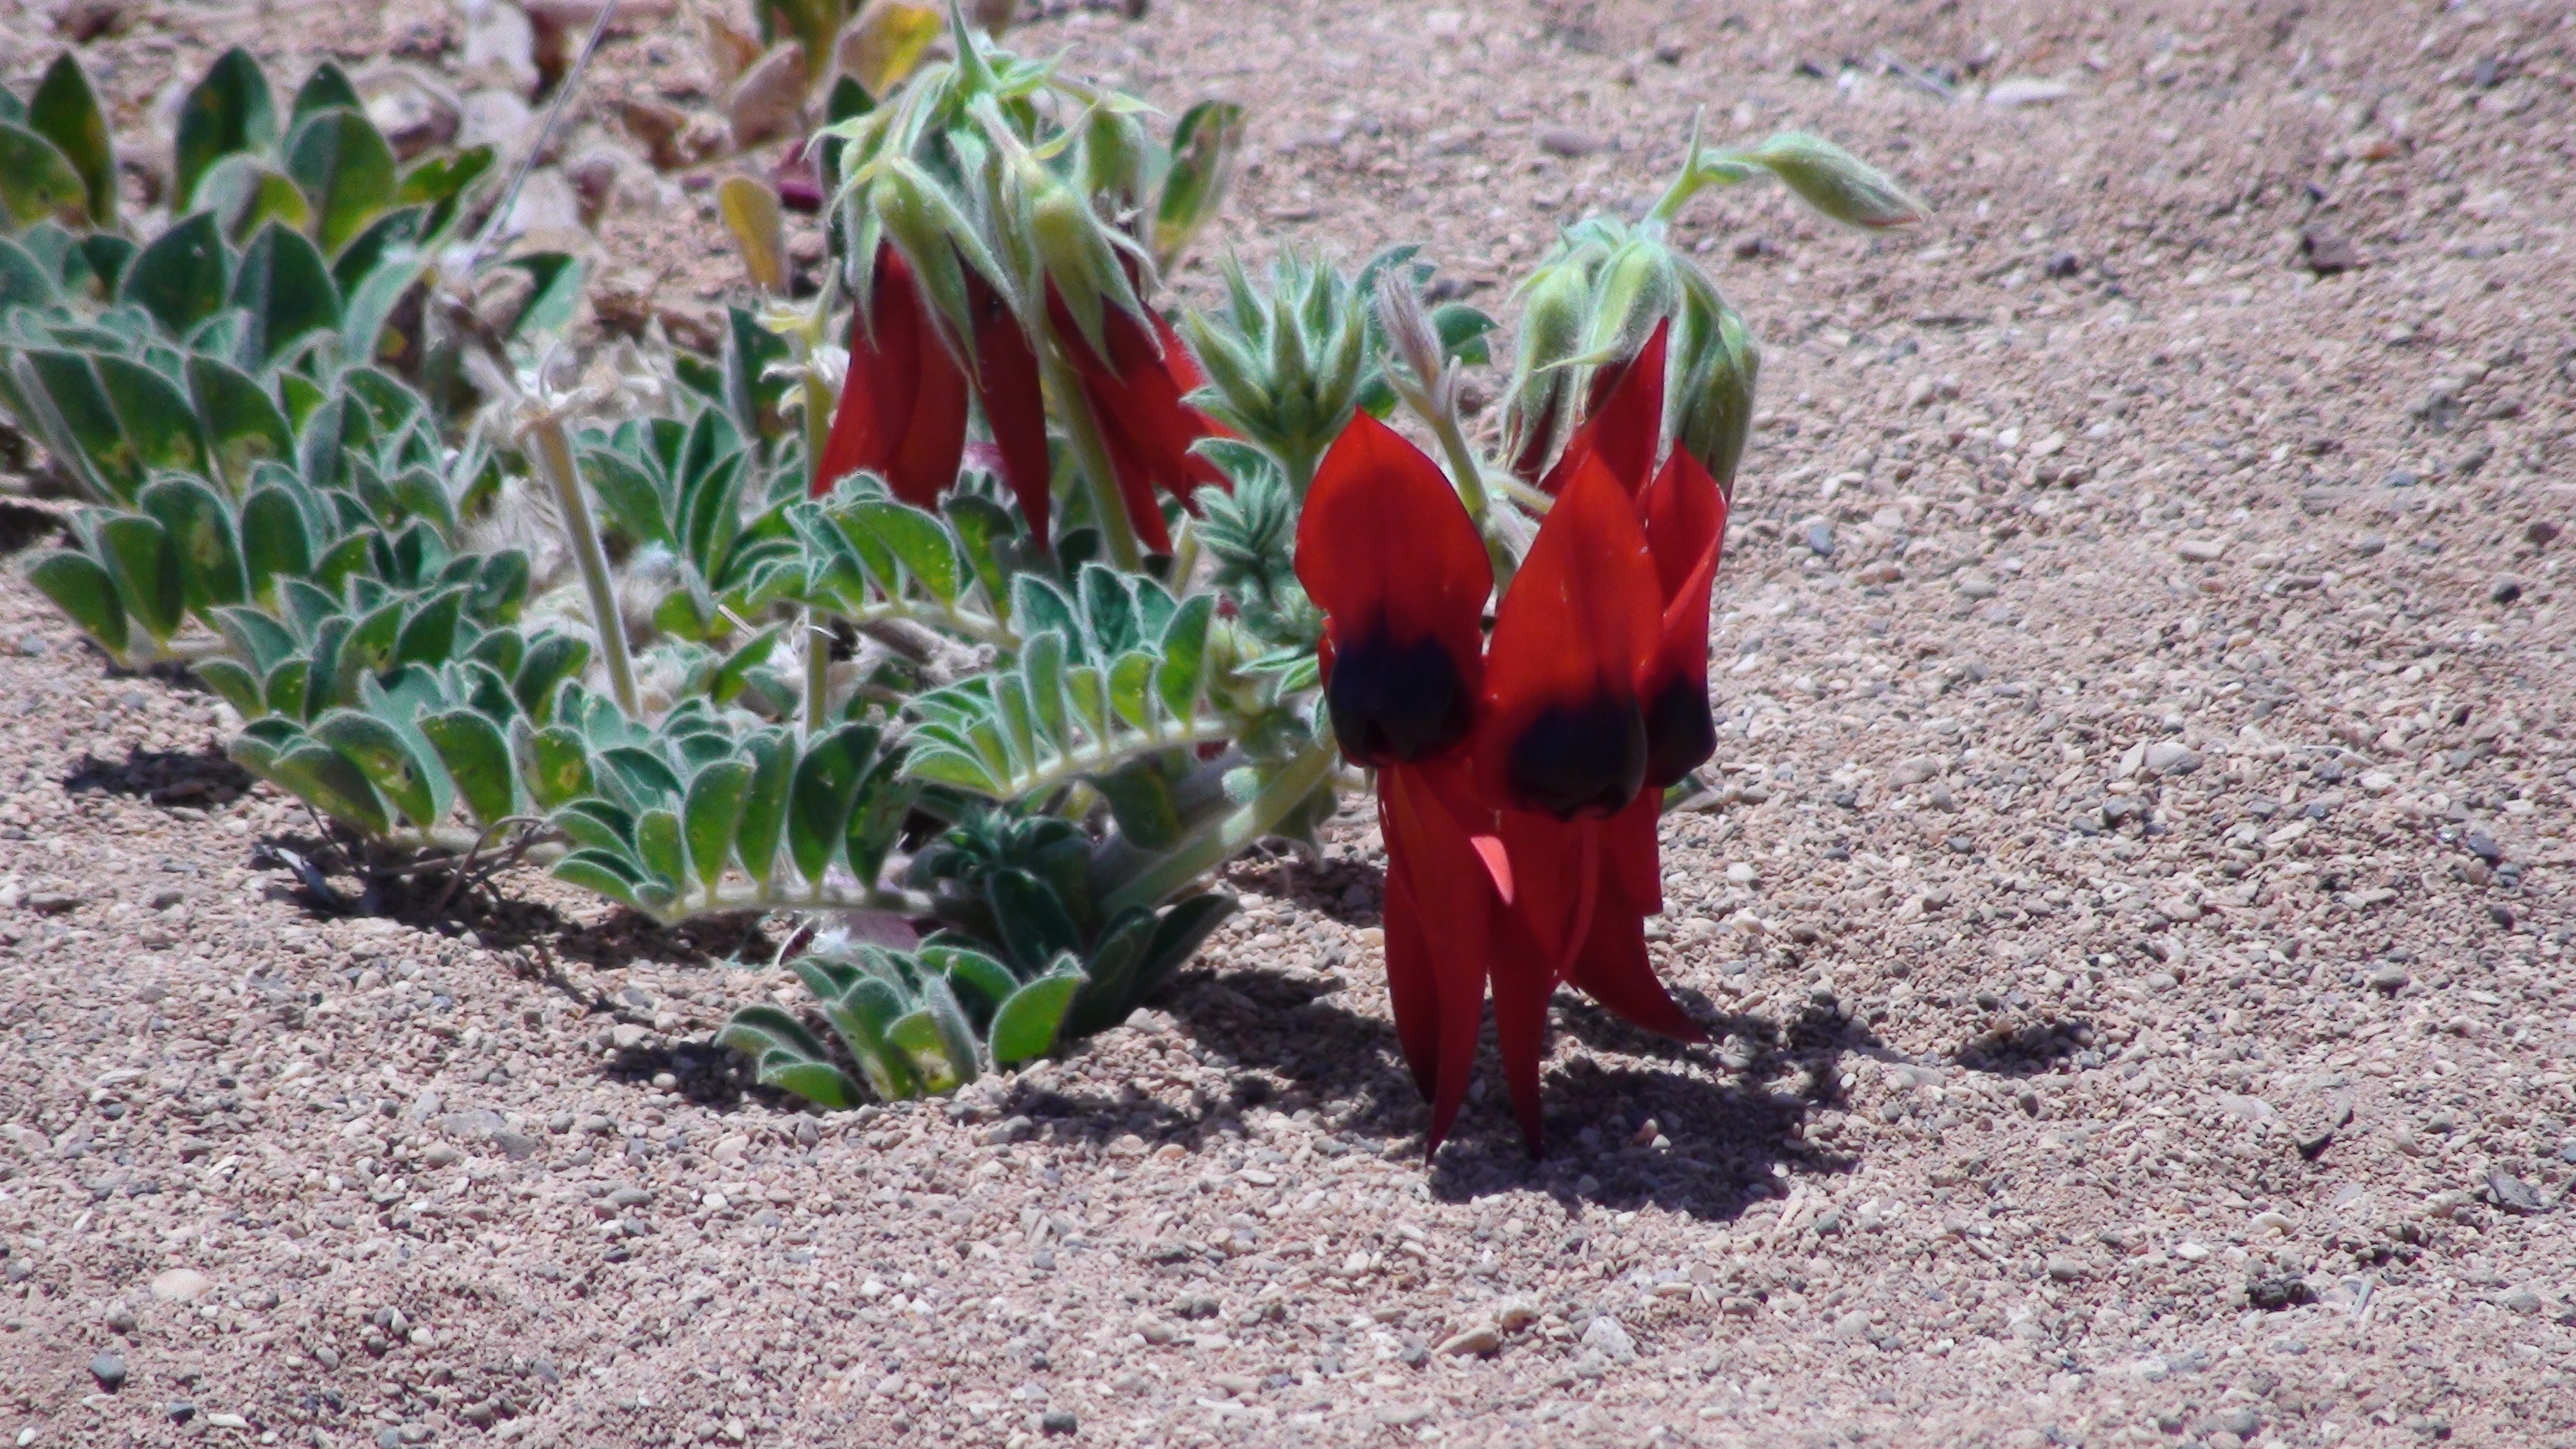
\includegraphics[angle=45,width=4in]{flower}

\end{document}
